\documentclass{article}
\usepackage{a4wide}
\usepackage{amssymb}
\usepackage{amsmath}
\usepackage[numbers]{natbib}
\usepackage{xcolor}
\usepackage[colorlinks,linkcolor=blue,urlcolor=blue,citecolor=blue]{hyperref}
\usepackage{mathrsfs}
\usepackage{comment}
\usepackage{tabularx}
\usepackage{booktabs}
\usepackage{caption}% http://ctan.org/pkg/caption
\captionsetup[table]{justification=raggedright, singlelinecheck=off}
\usepackage{amsthm}
\theoremstyle{definition}
\usepackage{pgf}
\usepackage{tikz}
\usetikzlibrary{arrows,automata}

\usepackage{tikz}
\usetikzlibrary{calc,positioning,shapes,arrows,decorations.pathreplacing}
\usetikzlibrary{shapes.multipart}


\title{Resource Constrained Project Scheduling for continuous applications using Precedence Constraint Posting.}
\author{M. van Gelderen  \and
    R.M. de Lange \and
    B. Gris\`el \and
    F. van Tienen}
\date{}

\pagestyle{empty}

\newcommand{\TODO}[1]{{\color{red}\textbf{TODO: #1}}}
\newtheorem{example}{Example}[section]

\newcommand{\res}[0]{\ensuremath{R}} %resources
\newcommand{\av}[2]{\ensuremath{av(r_{#1}, t_{#2})}} %availability of resource #1 at time #2
\newcommand{\capa}[1]{\ensuremath{cap(r_{#1})}} %capacity
\newcommand{\dur}[1]{\ensuremath{dur(v_{#1})}} %durability
\newcommand{\usage}[2]{\ensuremath{usage(v_{#1}, r_{#2})}} %usage of resource #2 by activity #1
\newcommand{\start}[1]{\ensuremath{start(v_{#1})}} %start time
\newcommand{\makespan}[1]{\ensuremath{C_{max}(#1)}} %makespan

\newenvironment{definition}[1][Definition]{\begin{trivlist}
\item[\hskip \labelsep {\bfseries #1}]}{\end{trivlist}}

\setlength{\parindent}{0pt}
\setlength{\parskip}{\baselineskip}

\begin{document}
\maketitle
\thispagestyle{empty}

\begin{abstract}
\TODO{rewrite when paper finished}
\end{abstract}


\newpage


\section{Scope and purpose}

In this paper we will discus the resource constraint project scheduling problem in practical applications.
Scheduling is a very common problem in many day-to-day applications, because many situations require a suitable schedule to define the order in which to perform different tasks.
Making a schedule proves to be a more complex process than one might expect, especially when complicating factors arise such as limited resources or a set deadline.
These factors can be taken into account to some extent by the resource constraint project scheduling problem.
Some other complicating factors may occur in practical applications, such as the possibility of break down of resources, delays or a growing set of tasks.
The scheduling problem is therefore, although it is quite common, one of the more complex problems in computer science.

This paper will deal with the scheduling problem, some complicating factors and the approximation of a solution to this problem in continuous applications.
In almost all practical application, an approximation is used to retrieve a schedule.
Although these approximations do not deliver the optimal solution to a problem, they often give a good working schedule in less time than an optimal solution.
For a continuous environment, this quick solution is key to keep up with the constant changes.

An approximation method will be discussed in light of the practical applications of the scheduling problem.
For the approximation simple temporal networks will be used, these allow to give a more simple representation of the complex scheduling problem.
Simple temporal networks are a form of graph representations using nodes and edges to represent the tasks, resources and constraints in the original scheduling problem.
One must note that this simpler representation does not allow for all scheduling problems to be represented correctly, therefore some solutions which are in fact feasible, might not be found using the approximation.

The purpose of this paper is to inform the reader on the topic of resource constraint scheduling in continuous applications.
The paper aims to be a good source of information on the topic of resource constraint scheduling and its link to the practical applications seen in daily life.
Although the reader is presumed to have prerequisite knowledge about for example set theory, graph theory, algorithmics and complexity theory, most in-depth information aims to be complete and clear.

%		-Wat staat waar?
In  chapter \ref{text:problem_background} \emph{Problem Background} we will first go deeper in to the resource constraint scheduling problem.
Here the different aspects of the resource constraint project scheduling problem will be discussed.
An example of a scheduling problem will be given, along with an intuitive description and formal definitions of the problem.
We will also look into the complexity \ref{text:complex} of the problem, showing why an approximation is needed for practical applications.

The following chapter, \ref{text:schedule} \emph{Schedule Construction}, will deal with the approximation of the solution.
For the approximation, simple temporal networks \ref{text:STN} will be used, which provide with a simpler way of representing a schedule.
The simple temporal networks will be explained using the example from the previous chapter and again giving an intuitive and formal definition.
When a more dynamic way of adjusting the schedule is required, precedence constraint posting \ref{text:PCP} is introduced to the simple temporal networks.
Precedence constraint posting is a technique which allows for changes to a temporal network by introducing new precedence constraints.
The workings of precedence constraint posting will also be explained using the example and giving an intuitive and formal definition.

Combining these two methods gives us a flexible way of approximating a resource constraint project scheduling problem.
Concluding we will show that this combination provides us with a solution capable of scheduling complex problems in continuous environments.
This gives us a robust and effective solution for scheduling in many practical applications.


\newpage


\section{Problem background}
\label{text:problem_background}

%		-What are scheduling problems?
In this chapter we will take a deeper look at the resource constraint project scheduling problem.
To do this, we will first discuss some real life examples and the use of the resource constraint project scheduling problem to get a more clear idea of the problem.
We will then give a running example, which will be used throughout this paper to make the problem more tangible.
Using this example, we will illustrate the formal definition of the resource constraint project scheduling problem.
With this formal definition and a good sense what the problem holds, the complexity of the problem will be discussed.

Before we go into the examples and definitions, let us first see what scheduling problems are.
Scheduling problems are problems in which several activities need to be put into a schedule.
For the execution of these activities, there is often a limited amount of resources available.
The schedule is called feasible when there is a solution that puts all activities in the schedule in such a way that they are all executable by the resources needed and do not overlap with conflicting tasks.
This is a simple form of scheduling, in the examples we will discuss further on more constraints will be added.
Such as for example the precedence constraint, in which one task needs to be finished before the other can start.
These extra constraints place more demands on the schedule for it to be feasible.

%		-Examples form real life.
An example of a real life application of the resource constraint project scheduling problem is train maintenance scheduling.
In scheduling the maintenance of trains, there are several factors which need to be taken into calculation.
For instance, the trains should not be out of service due to maintenance for too long of a period.
Also, there is limited space for trains to be serviced in the maintenance depot and not in every service bay all jobs can be performed.
There are service bays that maintain the electrical wiring or specialize in maintaining the wheels.
These factors make scheduling in an efficient way a complex task.

The same problems can be seen in other maintenance applications and also, for example, airport scheduling.
Airport scheduling has even more complicating factors, such as refueling, baggage handling, boarding and disembarking.
These are some complex examples to show that the problem has many difficult applications, but there exist simpler applications which require similar methods.
In the next section we will show a simple example using painters and some painting tasks, in which these complicating factors are represented and is still easily comprehensible when reading.

%		-What is RCPSP and how can it solve them.
%		-Why imporant.
%		-Voorbeelden wat meer uitwerken. Intuitief verhaal.
Now we have an idea about the uses of resource constraint scheduling, but what is it exactly?
The RCPSP concerns itself with finding start times for a set of activities so that the schedule is feasible and usually optimized in some way.
This optimization might be either the shortest processing time or the most efficient use of resources.
In this paper we will focus on the shortest processing time.
The scheduling problem consists of a few main elements: activities, resources and constraints.

Activities, also called tasks or jobs, are the tasks that need to be executed or jobs that need to be performed.
These activities are the elements that need to be scheduled in the first place.
Resources are the machines or personnel or equipment needed to perform a specific activity.
Resources can often perform a specific function and have a maximum capacity of simultaneous activities.
Constraints can be any number of limiting factors to which a specific activity, resource or entire schedule should hold.
For example, a constraint can be the fact that there is a limited number of one type of resource available (\emph{resource constraint}), or that one specific activity needs to be finished before another specific activity can be performed (\emph{precedence constraint}).

To illustrate the RCPSP, we will give a simplified example of the problem in the following section, using painters as a subject.

\subsection{RCPSP in general}

\TODO{c+p}

\subsection{Running example}
In this paper we will use a simple running example based on a painting job to explain the RCPSP. \TODO{uitweiden, \'e\'en zin als eerste alinea is een beetje schraal}

\TODO{Dit valt een beetje uit het niets, in de alinea kan je uitleggen dat we kijken naar een bedrijf dat opknap klusjes/renovaties doet. Er is een opdracht binnengekomen waarbij een huis opnieuw geschilderd moeten worden. We beschijven een versimpelde problemeinstantie uit de werkelijkheid voor dit \emph{schilderproject} (handig om naar te kunnen refereren misschien als je die term eens noemt)}
The problem consists of workers that need to finish three painting jobs: a door, a fence and a wall.
Because the the door and the fence are made of wood, both surfaces needs to be sanded first (\emph{precedence constraints}). \TODO{Ik vind het lelijk/ongepast om in een intuitieve definitie de termen tussen haakjes achter een vage beschrijving te zetten, gebruik het woord in de zin zoals je bij andere termen ook doet}
Sanding is not necessary for the wall, because the wall is made of bricks.
When the job is finished all painting brushes need to be cleaned and this can only be done when all the painting is finished.
This gives us six \emph{activities}: sanding the the door, sanding the fence,  painting the door, painting the fence, painting the wall and cleaning the painting brushes. \TODO{And aan het begin van de zin op deze manier lijkt me niet correct}
And the following precedence constraints: sanding the door before painting the door, sanding the fence before painting the fence and all the painting activities need to be done before cleaning the painting brushes.

Because the size of each surface in the painting jobs differs, not each activity takes the same amount of time to finish (\emph{duration}) \TODO{Idem}.
They define the duration for each of the activities in whole hours, because this makes it easier to schedule (\emph{time horizon}) \TODO{Na-ah}.
Since this is not the first painting job the workers have done, we assume that they know the exact duration for each activity \TODO{For simplicity's sake ipv because they are extremely experienced}:
\begin{itemize}
\item sanding the door: 3 hours
\item sanding the fence: 2 hours
\item painting the door: 2 hours
\item painting the fence: 1 hour
\item painting the wall: 5 hours
\item cleaning the painting brushes: 1 hour
\end{itemize}
\TODO{lijkt me geschikt om in een tabel te zetten met kolommen activity en hours of periods, kun je er ook naar refereren. Misschien nog float right om de tabel naast de alinea te krijgen maar dat is voor latere zorg}
% moet nog even goed gestyled worden

Normally this would be an easy job \TODO{vaag, wat is \emph{this}? Iets in de strekking van: "Normally there are enough tools available for everyone to work with. Unfortunately, the crew has a very limited amount of tools this time around." lijkt me beter} (\emph{resources}) \TODO{ verwerk in tekst}
So now they only have two painting brushes and one sanding machine (\emph{resource constraints}), which makes it impossible to sand more than one surface at the same time and to paint more than two surfaces at the same time.
This shows us that the \emph{capacity} of painting surfaces at the same time is two and the capacity of sanding surfaces at the same time is one.

Since every sanding job uses the sanding machine as a resource, the usage of sanding the door and sanding the fence is $1$ for the sanding machine. \TODO{Ik denk dat dit een vreemde manier van opschrijven is voor iemand die de notatie nog niet kent}
Also every painting job uses the painting brush as a resource, so that painting the door, painting the fence and painting the wall all have a usage of $1$ on the painting brush. \TODO{a usage of 1. Ik denk echt dat het volstaat om te noemen dat voor het uitvoeren van deze taken \'e\'en painting brush nodig is. }
There is only one activity left, cleaning the painting brushes, which will use both of the painting brushes resource so that the usage on the painting brushes is $2$.
Because a sanding activity doesn't use a painting brush, a painting activity doesn't use a sanding machine and cleaning the painting brushes doesn't use a sanding machine all of the other usages are $0$. \TODO{same story}

The painters want to make a schedule, where they define each starting time for the activities in such a way that the resulting schedule is feasible. \TODO{Splits dit in meer zinnen, 1: they want to make a schedule to complete the project 2: they define the schedule by assinging a start time to each .. 3: requirements for the schedule is that the the sanding happens before the painting, and the painting before the cleaning. 4: it also must keep the limited amount of tools in mind. }
This means that the sanding of each wooden surface (the door and the wall) needs to be finished before starting the painting of that surface.
Because of the limited resources, they can never paint more than two surfaces at once nor can they sand more than one surface at once. 
\TODO{Describe in terms of projects instead of jobs, here you can refer to the painting project (earlier todo)} There are also a lot of other jobs to do, so the painter not only want a feasible schedule but also want to optimize the time in which they finish all the activities. \TODO{what kind of optimization? I know what you mean but I shouldn't have to think about it first in the intuitive definition}

\subsection{Definition \TODO{Definition is meer Notation imo}}
\label{text:definitions}

\TODO{ik zou een paragraaf niet beginnen met een plaatje}

\begin{figure}[ht]
	\centering
	% Author: Mick van Gelderen
% Created from http://www.texample.net/tikz/examples/class-diagram/ and other examples and resources. 

%\documentclass{standalone}
%\usepackage{tikz}
\usetikzlibrary{calc,positioning,shapes,arrows,decorations.pathreplacing}
\usetikzlibrary{shapes.multipart}


%\begin{document}

\tikzstyle{activity}=[rectangle, draw=black, text centered, text=black, thick, minimum height=1.8em, minimum width=1.8em]
\tikzstyle{dummy}=[rectangle, fill=black!7, draw=black, text centered, text=black, thick, minimum height=1.8em, minimum width=1.8em]
\tikzstyle{precedence}=[->,>=stealth, draw=black!70, thick]

\newcommand{\activity}[3]{\node (v#1) [activity, text width=#2cm, #3] {$v_#1$};}

\begin{tikzpicture}[node distance=.8cm]
		\node (v0) [dummy] {$v_0$};
    \activity{2}{2}{right=1.6cm of v0}
    \activity{1}{3}{above=of v2}
    \activity{3}{2}{right=of v1}
    \activity{4}{1}{below=of v3}
    \activity{5}{5}{below=of v2}
    \activity{6}{1}{right=1.6cm of v4}
		\node (v7) [dummy, right=of v6] {$v_7$};
		
    \draw[precedence] (v0.east) to[out=0,in=180] (v1.west);
    \draw[precedence] (v0.east) to[out=0,in=180] (v2.west);
    \draw[precedence] (v0.east) to[out=0,in=180] (v5.west);
    \draw[precedence] (v1.east) to[out=0,in=180] (v3.west);
    \draw[precedence] (v2.east) to[out=0,in=180] (v4.west);
    \draw[precedence] (v3.east) to[out=0,in=180] (v6.west);
    \draw[precedence] (v4.east) to[out=0,in=180] (v6.west);
    % start bending from the projection v4 on the line y=v3.y
    \draw[precedence] (v5.east) -- ($(v5)!(v4)!($(v5)+(1,0)$)$) to[out=0,in=180] (v6.west);
		\draw[precedence] (v6.east) to[out=0,in=180] (v7.west);		    

    % Descriptions
    \path (v3.east) to[out=0,in=180] coordinate (temp) (v6.west);
    \draw[shorten <=2pt, shorten >=2pt] (temp) -- ++(.8,.6) node[anchor=west, yshift=2pt, text width=2cm] {Precedence constraint $(v_3, v_6) \in E$};
    
    \draw[shorten <=2pt, shorten >=2pt] (v5.south) -- ++(.8,-.6) node[anchor=west, yshift=-2pt] {Activity $v_5$};
    
    % Funky braces
    \draw[decorate,decoration={brace,amplitude=8pt}]
        let \p1 = (v5.west), \p2 = (v6.east), \p3 = (v1) in 
        (\x1, \y3+1cm) -- (\x2, \y3+1cm) node[midway, above=10pt] {$V = \{v_1, \ldots, v_6\}$};
        
    \draw[decorate,decoration={brace,amplitude=8pt}]
        let \p1 = (v0.west), \p2 = (v7.east), \p3 = (v1) in 
        (\x1, \y3+2cm) -- (\x2, \y3+2cm) node[midway, above=10pt] {$W = V \cup \{v_0, v_7\}$};
    
\end{tikzpicture}

%\end{document}
	\caption{The activity graph for the running example. \TODO{"The" weglaten?}}
	\label{fig:activity_graph}
\end{figure}

The \emph{time horizon} is a mapping of real-world time to model-time is indicated by the so called time horizon $T \in \mathbb{N}$.
The periods within the time horizon $t=1,2,3,\ldots,T$ are also notated as $t_j$ which means the $j$-th time period in the time horizon $T$. 
The time period $t_j$ corresponds to the time interval $(t-1,t]$. 
\TODO{Make a reference to a figure}

\emph{Activities} are specified by a set $V = \{v_1, \ldots, v_n\}$. \TODO{each element $v_i$ from this set represents the i-th activity of the project? ipv identifier?}
This is a set of activities where the total amount of activities is $n \in \mathbb{N}$ \TODO{$n = |V|$?} and each activity is represented by a unique identifier. %identifier??
In the running example we have six activities: sanding the the door $v_1$, sanding the fence $v_2$,  painting the door $v_3$, painting the fence $v_4$, painting the wall $v_5$ and cleaning the painting brushes $v_6$. 
Which gives us the total set of activities $V = \{v_1, \ldots, v_6\}$ with $n = 6$ for the running example.
These activities are represented in Figure \ref{fig:activity_graph} as blocks.

The \emph{duration} for each activity $v_i \in V$ is specified by $\dur{i} \in \mathbb{N}$.
In the running example the activities have the following duration: $\dur{1} = 3, \dur{2} = 2, \dur{3} = 2, \dur{4} = 1, \dur{5} = 5, \dur{6} = 1$. \TODO{reference usage diagram for the activities with their durations?}

The duration of each activity in the running example is represented by the length of the block in Figure \ref{fig:activity_graph}.

\TODO{Discuss W here as well and the reason why their blocks are filled with a shade of gray. You can do it before discussing the precedence constraints because you have already talked about activities anyway}

\emph{Precedence constraints} are specified by a set $E = \{(v_i, v_j) | v_i \in V, v_j \in V, v_i \neq v_j\}$ \TODO{Volgens mij wilde cees ipv $\neq$ juist $v_i < v_j$, zie aantekeningen}
This means that a precedence relation between activities $v_i$ and $v_j$, where $v_j$ can be started only after $v_i$ is finished, is represented as $(v_i, v_j) \in E$.
The running example has several precedence constraints between the activities, which make up the following set $E = \{(v_1, v_3), (v_2, v_4), (v_3, v_6), (v_4, v_6), (v_5, v_6)\}$.
\TODO{Discuss the precedence constraints of the dummy activities here}
Figure \ref{fig:activity_graph} shows the precedence constraints for the running example, represented as arrows between the nodes.
\TODO{Explain why there is no precedence ($v_0$, $v_6$) for example in the illustration}

\TODO{MOVE UP}
The \emph{extended activity set} is specified by $W = V \cup \{v_0, v_{n+1}\}$.
Which consists of the activity set $V$ and incorporates a unique dummy beginning activity $v_0$ and a unique dummy ending activity $v_{n+1}$. 
These dummy activities have a duration of $0$ periods.
Precedence constraints are added to ensure that the starting activity starts before every other activity and that every activity is completed before the ending activity. 
For the running example we will have a set $W = \{v_0, \ldots v_7\}$. \TODO{Ik denk dat "will have" hier een beetje nederengels is}
Figure \ref{fig:activity_graph} shows $W$ for the running example. 

The \emph{constraints graph} is specified by a directed graph $G = (V, E)$.
It consists of the activities $V$, which are represented as nodes, and the precedence constraints $E$, which are represented as connections between nodes.
The constraints graph for the running example is represented in Figure \ref{fig:activity_graph}, where the precedence constraints are reduced to a minimum. \TODO{Dit stukje moet misschien eerder ofzo?}

\begin{figure}[h]
	\centering
	% Author: Mick van Gelderen
% Created from http://www.texample.net/tikz/examples/class-diagram/ and other examples and resources. 

%\documentclass{standalone}
%\usepackage{tikz}
\usetikzlibrary{calc,positioning,shapes,arrows,decorations.pathreplacing}
\usetikzlibrary{shapes.multipart}


%\begin{document}




\newcommand{\activity}[3]{\node (v#1) [activity, text width=#2cm, #3] {$v_#1$};}

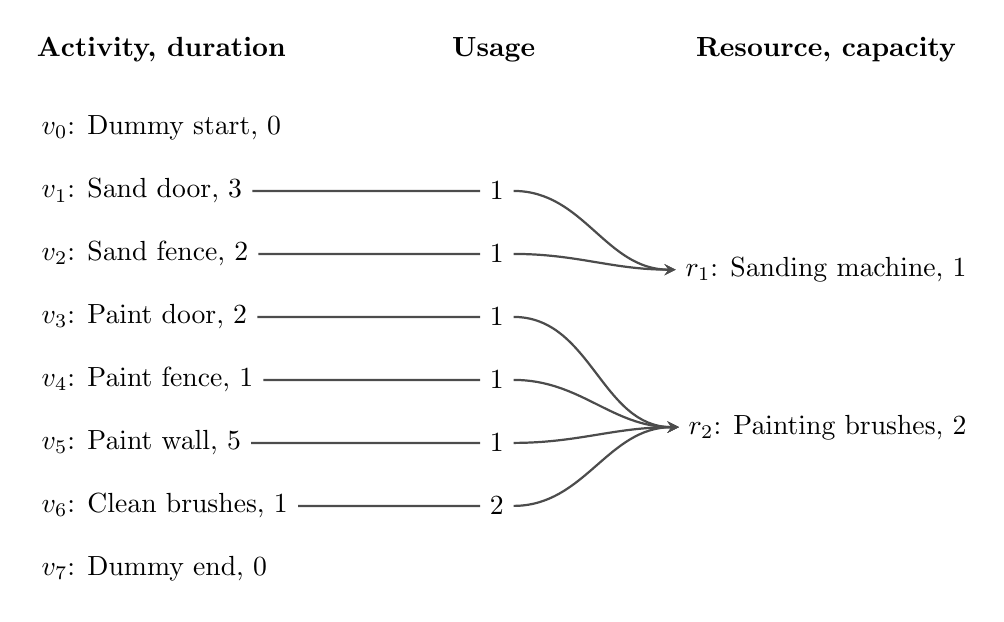
\begin{tikzpicture}[node distance=.8cm]
	\tikzstyle{activity}=[text centered, text=black, thick, minimum height=1.8em, minimum width=1.8em]
	\tikzstyle{resource}=[text centered]
	\tikzstyle{header}=[font=\bfseries]
	\tikzstyle{usage}=[->,>=stealth, draw=black!70, thick]

	\node (v0) [activity] {$v_0$: Dummy start, 0};
	\node (v1) [activity, below=of v0.west, anchor=west] {$v_1$: Sand door, 3};
	\node (v2) [activity, below=of v1.west, anchor=west] {$v_2$: Sand fence, 2};
	\node (v3) [activity, below=of v2.west, anchor=west] {$v_3$: Paint door, 2};
	\node (v4) [activity, below=of v3.west, anchor=west] {$v_4$: Paint fence, 1};
	\node (v5) [activity, below=of v4.west, anchor=west] {$v_5$: Paint wall, 5};
	\node (v6) [activity, below=of v5.west, anchor=west] {$v_6$: Clean brushes, 1};
	\node (v7) [activity, below=of v6.west, anchor=west] {$v_7$: Dummy end, 0};
	
	\node (u1) [right=5.7cm of v1.west] {1};
	\node (u2) [right=5.7cm of v2.west] {1};
	\node (u3) [right=5.7cm of v3.west] {1};
	\node (u4) [right=5.7cm of v4.west] {1};
	\node (u5) [right=5.7cm of v5.west] {1};
	\node (u6) [right=5.7cm of v6.west] {2};

	\coordinate (mid) at ($(v0.west)!.5!(v7.west) + (12,0)$);
	\node (r1) [resource, above=1cm of mid, anchor=east] {$r_1$: Sanding machine, 1};
	\node (r2) [resource, above=-1cm of mid, anchor=east] {$r_2$: Painting brushes, 2};

	\draw let \p1 = (v0), \p2 = (r1) in 
		node (ac) [header] at ($(\x1,\y1) + (0,1)$) {Activity, duration}
		node (res) [header] at ($(\x2,\y1) + (0,1)$) {Resource, capacity};
	\node (us) [header] at ($(ac)!.5!(res)$) {Usage};
	
  \draw[usage] (v1.east) -- (u1) to[out=0,in=180] (r1.west);
  \draw[usage] (v2.east) -- (u2) to[out=0,in=180] (r1.west);
  \draw[usage] (v3.east) -- (u3) to[out=0,in=180] (r2.west);
  \draw[usage] (v4.east) -- (u4) to[out=0,in=180] (r2.west);
  \draw[usage] (v5.east) -- (u5) to[out=0,in=180] (r2.west);
  \draw[usage] (v6.east) -- (u6) to[out=0,in=180] (r2.west);

  
	
\end{tikzpicture}

%\end{document}
	\caption{Activities, resources and the relation between them for the running example. }
	\label{fig:resource_graph}
\end{figure}

\emph{Resources} are specified by a set $R = \{r_1, \ldots, r_m\}$.
The total amount of resources is $m \in \mathbb{N}$ and each resource is represented by a unique identifier. %identifier??
In the running example we have two resources ($m = 2$): the sanding machine $r_1$ and the painting brushes $r_2$.
Which gives us the total set of resources $R = \{r_1, r_2\}$.
In Figure \ref{fig:resource_graph} and in Figure \ref{fig:feasible_schedule} you will see all the resources of the running example. \TODO{informeel}

The \emph{capacity} of each resource $r_i \in R$ is specified by a function $\capa{i} \in \mathbb{N}$.
For the running example we the capacity for resources are: $\capa{1} = 1, \capa{1} = 2$. \TODO{hmm?}
These capacities are shown in Figure \ref{fig:resource_graph} and in Figure \ref{fig:feasible_schedule}, represented as the height for each resource. 

The \emph{usage} of an activity $v_i \in V$ consumes of a resource $r_j \in \res$ during its execution is specified by the function $\usage{i}{j} \in \mathbb{N}$.
The running example has the following usages: $\usage{1}{2} = 1, \usage{2}{2} = 1, \usage{3}{1} = 1, \usage{4}{1} = 1, \usage{5}{1} = 1, \usage{6}{1} = 2$.
Figure \ref{fig:resource_graph} shows the usages as relations between activities and resources. \TODO{reformulate}

Figure \ref{fig:feasible_schedule} shows us the usages represented as hight for each activity. \TODO{what si this doing here?}

\TODO{introduce the time feasible schedule here shortly}
\begin{figure}[h]
	\centering
	% Author: Mick van Gelderen
% Created from http://www.texample.net/tikz/examples/class-diagram/ and other examples and resources. 

%\documentclass{standalone}
%\usepackage{tikz}
\usetikzlibrary{calc,positioning,shapes,arrows,decorations.pathreplacing}
\usetikzlibrary{shapes.multipart}


%\begin{document}

% This file is included by preamble.tex from base directory ../

\pgfdeclarepatternformonly{swnestripes} {
	\pgfpoint{0cm}{0cm}
}{
	\pgfpoint{2cm}{2cm}
}{
	\pgfpoint{1cm}{1cm}
}{
		\pgfsetlinewidth{10pt}
		\pgfpathmoveto{\pgfpoint{0cm}{0cm}}
		\pgfpathlineto{\pgfpoint{2cm}{2cm}}
		\pgfusepath{stroke}
}

% SICKE SHIT YEAA!
\pgfdeclarepatterninherentlycolored{sandingpainting} {
	\pgfpoint{0cm}{0cm}
}{
	\pgfpoint{4cm}{4cm}
}{
	\pgfpoint{2cm}{2cm}
}{
		\pgfsetlinewidth{10pt}
		\pgfsetcolor{orange!28}
		\pgfpathmoveto{\pgfpoint{0cm}{0cm}}
		\pgfpathlineto{\pgfpoint{10cm}{10cm}}
		\pgfpathclose%
		\pgfusepath{stroke}
		\pgfsetcolor{blue!14}
		\pgfpathmoveto{\pgfpoint{1cm}{0cm}}
		\pgfpathlineto{\pgfpoint{11cm}{10cm}}
		\pgfpathclose%
		\pgfusepath{stroke}
}

\tikzstyle{activity}=[rectangle, draw=black, anchor=south west, minimum height=1cm, minimum width=1cm]
\tikzstyle{sanding}=[pattern=swnestripes, pattern color=orange!28]
\tikzstyle{painting}=[pattern=swnestripes, pattern color=blue!14]
\tikzstyle{sandingpainting}=[pattern=sandingpainting]

\tikzstyle{invalid}=[draw=red, ultra thick]
\tikzstyle{axis}=[->,thick,>=stealth,shorten >=-.3cm,shorten <=-.3cm]
\tikzstyle{yaxisnode}=[text depth=0pt, text height=2ex, rotate=90, yshift=3.7ex, anchor=north east]
\tikzstyle{capacity}=[dashed,shorten >=-.3cm, shorten <=-.3cm]

\begin{tikzpicture}[node distance=1]
    \draw[axis] (0,0) -- (6,0) node[anchor=north, yshift=-1em] {Time};
		\draw[axis] (0,0) -- (0,3) node[yaxisnode] {Activities};
    \node (v1) [activity, minimum width=3cm] at (0,2) {$v_1$};
\node (v2) [activity, minimum width=2cm] at (0,1) {$v_2$};
\node (v3) [activity, minimum width=2cm] at (3,2) {$v_3$};
\node (v4) [activity, minimum width=1cm] at (2,1) {$v_4$};
\node (v5) [activity, minimum width=5cm] at (0,0) {$v_5$};
\node (v6) [activity, minimum width=1cm] at (5,0) {$v_6$};

\draw[dotted] (v2.south east) -- ++(0,-1) node[anchor=north] {$t_2$};
\draw[dotted] (v4.south east) -- ++(0,-1) node[anchor=north] {$t_3$};
\node [anchor=north west] at (0,0) {$t_0$};
\node [anchor=north] at (5,0) {$t_5$};
\node [anchor=north] at (6,0) {$t_6$};
\end{tikzpicture}

%\end{document}
	\caption{A time feasible schedule for the running example. }
	\label{fig:time_feasible_schedule}
\end{figure}

\TODO{use fig:time\_feasible\_schedule to explain what a schedule is, what the makespan, feasability and mabye availability}
\TODO{I do not see a use for availability to be honest but whatever}

A \emph{schedule} is specified by a set $S = \{\start{1}, \ldots, \start{n}\}$.
For the running example a possible schedule is shown in Figure \ref{fig:time_feasible_schedule}.

The \emph{makespan} of a schedule $S$ is the number of periods required to finish the project using the schedule $S$. The makespan is notated as $\makespan{S} \in T$.
In the running example we can create a time feasible schedule (shown in Figure \ref{fig:time_feasible_schedule}) \TODO{dont you parenthesis on me again}, where the makespan is optimized to a minimum and all the precedence constraints hold. 

\begin{figure}[h]
	\centering
	% Author: Mick van Gelderen
% Created from http://www.texample.net/tikz/examples/class-diagram/ and other examples and resources. 

%\documentclass{standalone}
%\usepackage{tikz}
\usetikzlibrary{calc,positioning,shapes,arrows,decorations.pathreplacing}
\usetikzlibrary{shapes.multipart}


%\begin{document}

\tikzstyle{activity}=[rectangle, draw=black, anchor=south west, minimum height=1cm, minimum width=1cm]
\tikzstyle{invalid}=[fill=black!8]
\tikzstyle{axis}=[->,thick,>=stealth,shorten >=-.3cm,shorten <=-.3cm]
\tikzstyle{capacity}=[dashed,shorten >=-.3cm, shorten <=-.3cm]
\begin{tikzpicture}[node distance=1, scale=1, every node/.style={transform shape}]

  \begin{scope}[shift={(7,0)}]
    \draw[axis] (0,0) -- (6,0);% node[anchor=north, yshift=-1em] {Time};
    \draw[axis] (0,0) -- (0,3);% node[anchor=north east] {Activities};

    \node (v1) [activity, minimum width=3cm] at (0,1) {$v_1$};
    \node (v2) [activity, minimum width=2cm] at (3,2) {$v_2$};
    \node (v3) [activity, minimum width=2cm] at (3,1) {$v_3$};
    \node (v4) [activity, minimum width=1cm] at (5,2) {$v_4$};
    \node (v5) [activity, minimum width=5cm] at (0,0) {$v_5$};
    \node (v6) [activity, minimum width=1cm] at (5,0) {$v_6$};

    \draw[dotted] (v3.south west) -- ++(0,-1) node[anchor=north] {$t_3$};
    \node [anchor=north west] at (0,0) {$t_0$};
    \node [anchor=north] at (5,0) {$t_4$};
    \node [anchor=north] at (6,0) {$t_6$};
  \end{scope}
  
\end{tikzpicture}

%\end{document}
	\caption{\TODO{A schedule that shows the exceeding in resources in the time schedule for the running example.} }
	\label{fig:fail_schedule}
\end{figure}

The \emph{availability} of an activity $v_i \in V$ at a time $t_j \in T$ is specified by a function $\av{i}{j} \in \mathbb{N}$.
For example if you only paint one object in the running example at $t_1$, the availability of $r_2$ is $\av{2}{1} = 1$ because we have two painting brushes and only one is used.
In Figure \ref{fig:feasible_schedule} the availability of a resource can be deduced as the total hight of a resource minus all the activities that uses the resource. 

\begin{figure}[h]
	\centering
	% Author: Mick van Gelderen
% Created from http://www.texample.net/tikz/examples/class-diagram/ and other examples and resources. 

%\documentclass{standalone}
%\usepackage{tikz}
\usetikzlibrary{calc,positioning,shapes,arrows,decorations.pathreplacing}
\usetikzlibrary{shapes.multipart}


%\begin{document}

\tikzstyle{activity}=[rectangle, draw=black, anchor=south west, minimum height=1cm, minimum width=1cm]
\tikzstyle{invalid}=[fill=black!8]
\tikzstyle{axis}=[->,thick,>=stealth,shorten >=-.3cm,shorten <=-.3cm]
\tikzstyle{capacity}=[dashed,shorten >=-.3cm, shorten <=-.3cm]
\begin{tikzpicture}[node distance=1, scale=1, every node/.style={transform shape}]

  \begin{scope}[shift={(7,0)}]
    \draw[axis] (0,0) -- (6,0);% node[anchor=north, yshift=-1em] {Time};
    \draw[axis] (0,0) -- (0,3);% node[anchor=north east] {Activities};

    \node (v1) [activity, minimum width=3cm] at (0,1) {$v_1$};
    \node (v2) [activity, minimum width=2cm] at (3,2) {$v_2$};
    \node (v3) [activity, minimum width=2cm] at (3,1) {$v_3$};
    \node (v4) [activity, minimum width=1cm] at (5,2) {$v_4$};
    \node (v5) [activity, minimum width=5cm] at (0,0) {$v_5$};
    \node (v6) [activity, minimum width=1cm] at (5,0) {$v_6$};

    \draw[dotted] (v3.south west) -- ++(0,-1) node[anchor=north] {$t_3$};
    \node [anchor=north west] at (0,0) {$t_0$};
    \node [anchor=north] at (5,0) {$t_4$};
    \node [anchor=north] at (6,0) {$t_6$};
  \end{scope}
  
\end{tikzpicture}

%\end{document}
	\caption{\TODO{A feasible schedule $S_f$ for the running example.} }
	\label{fig:feasible_schedule}
\end{figure}

\subsection{Formal definition of the running example}

In Example \ref{exmp:running} we define the formal definition of the \emph{Running Example} by using the definitions in subsection \ref{text:definitions}.
\begin{example}
\label{exmp:running}
$V = \{v_1, \ldots, v_6\}$\\
$E = \{(v_1, v_3), (v_2, v_4), (v_3, v_6), (v_4, v_6), (v_5, v_6)\}$\\
$R = \{r_1, r_2\}$\\
$\dur{1} = 3, \dur{2} = 2, \dur{3} = 2, \dur{4} = 1, \dur{5} = 5, \dur{6} = 1$\\
$\usage{1}{2} = 1, \usage{2}{2} = 1, \usage{3}{1} = 1, \usage{4}{1} = 1, \usage{5}{1} = 1, \usage{6}{1} = 2$\\
$\capa{1} = 2, \capa{2} = 1$
\end{example}


\subsection{RCPSP formal definition}

\begin{definition}
Given:
A set of activities $V = v_1, \ldots, v_n$, a set of resources $R = \{r_1, \ldots, r_m\}$ and a set of precedence constraints $E =  \{(v_i, v_j) | v_i \in V, v_j \in V, v_i \neq v_j\}$.
Where each activity $v_i \in V$ has a duration $\dur{i} \in \mathbb{N}$ and each resource $r_j \in R$ has a capacity $\capa{j} \in \mathbb{N}$. 
And each activity $v_i \in V$ can use the capacity of a resource $r_j \in R$ with usage $\usage{i}{j} \in \mathbb{N}$.

Find:
A feasible schedule $S_f = \{s_1, \ldots s_n\}$, consisting of starting times for the activities in $V$.
Where each precedence constraint in $E$ holds, denoted by $\forall (v_i, v_j) \in E (\start{i} + \dur{i} \leq \start{j})$.
And no resource exceeds its capacity in usage at any time in the schedule, denoted by $\forall r_i \in R, t_j \in T (0 \leq \av{i}{j})$.
\end{definition}


\subsection{Complexity of the RCPSP}
\label{text:complex}
\TODO{Freek: complexiteit en oplosbaarheid.}
%		-Wat zijn de voor en nadelen van heuristic (niet optimaal, eigenlijk is het best kut maar we kunnen niet anders)}


\newpage


\section{Schedule construction}
\label{text:schedule}

As shown, the RCPSP is a complex problem, to find an optimal solution exponential time is needed.
In order to find a solution to the RCPSP in a more timely manner, we use an approximation.
In this chapter we will introduce this approximation, in the form of a \emph{Simple Temporal Network}, or STN.
After which a reduction of the RCPSP to a STN is given.
The STN graph gives a representation of the scheduling problem, considering the activities, resources and constraints given in the original problem.
We will then take a look at the resources and a method to post new activities and constraints to the created STN, using precedence constraint posting.
The resulting schedule representation is flexible and robust, which makes it very useful for continuous applications.

%		-Wat gaan we benaderen (relevantie van STN)
The use of an STN to approximate an RCPSP is specifically practical, while the STN allows us to save multiple starting times per activity.
This makes the STN more of a collection of feasible schedules, which gives the schedule represented by it extra flexibility.
Furthermore, the simple temporal problem is a problem which is quite similar to path finding and is thus solvable in polynomial time.
These two important features make the STN a useful approximation of the RCPSP, which is neither flexible, nor solvable in polynomial time.

%		-Geen volledige reductie, dus niet alle instanties worden chill afgebeeld 
The STN does not completely represent the original RCPSP, but is just an approximation.
There are cases in which the RCPSP is feasible, but using an STN will not give a working schedule.
\TODO{wat zijn deze gevallen? Hebben we een voorbeeld? Of laten we dat weg?}
This is an important shortcoming of this approximation.
Given the advantages in speed and flexibility, this shortcoming has to be taken for granted in using RCPSP in a dynamic environment.

\subsection{Simple Temporal Problem}
\label{text:STN}
Let us first introduce a notion of such a \emph{Simple Temporal Network} (STN) using a basic example. 
Note that the problem in question is called a \emph{Simple Temporal Problem} (STP) which is represented using an STN.

\subsubsection{Example}
\begin{example}
\label{exmp:stn}
Consider the following events which may occur on a typical work day:
\begin{enumerate}
\item I left my home between 8:05 and 8:10
\item After driving for 20 minutes, I had to stop for an open bridge
\item I waited for 5 to 10 minutes at the bridge
\item At 8:30, I arrived at work 
\end{enumerate}
\end{example}

Question we would now like to ask ourselves are: ``is this information consistent?'' and ``At what time(s) could I have left my home such that the above story would be true?''. 
Suppose I would have left at 8:10 and drove for 20 minutes and waited 5 minutes at the bridge, I would have arrived at work at 8:35, while I stated that I had arrived at work exactly at 8:30. 
Given the above constraints, it is not hard to discover that the only possible scenario is that I left home at 8:05 and waited only 5 minutes at the bridge.
The challenge now is to implement an algorithm that performs the same kind of reasoning. This can be done by regarding this problem as an STP and represent it using a STN.

\subsubsection{Constraint Graph}
The first step is to represent the example above as a \emph{constraint graph}. 
The nodes in this graph correspond to the events in the story and a directed edge from node $n_i$ to $n_j$ indicates that the event represented by node $n_i$ has to occur before the event represented by node $n_j$.
These edges are called \emph{constraints}. Additionally, each edge $(n_i, n_j)$ has got a certain \emph{time window} associated with it, which indicates the minimum and maximum delay between the two events represented by time points $n_i$ and $n_j$. 
Each node in this graph is called a \emph{time point}. 
An additional time point is added and refers to \emph{time zero}. This node is connected to the node that represents the activity with the latest start time.
A convenient time zero for this example is 8:00.
The constraint graph for this example is shown below. 

\begin{figure}[h]
	\centering
	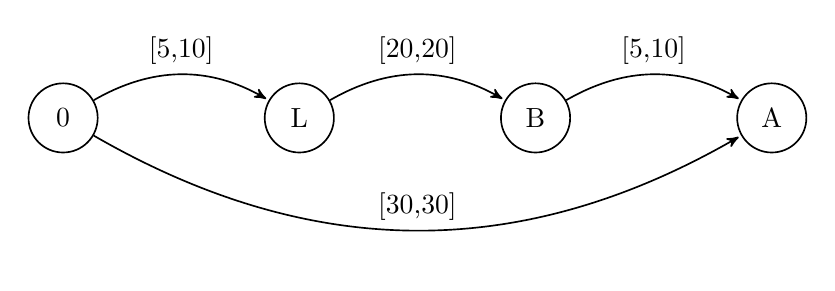
\begin{tikzpicture}[
		->,
		>=stealth',
		shorten >=1pt,
		auto,
		node distance=3cm,
	     semithick
	  ]
	
	  \node[state] (1) 						{0};
	  \node[state] (2) [right of=1] 		{L};
	  \node[state] (3) [right of=2] 		{B};
	  \node[state] (4) [right of=3] 		{A};
	
	  \path 	 (1) 	edge [bend left]    	node {[5,10]} 		(2)
	            		edge [bend right] 		node {[30,30]} 	(4)
	       	 (2) 	edge [bend left]		node {[20,20]} 	(3)
	        	 (3) 	edge [bend left]     	node {[5,10]} 		(4);
	        
	\end{tikzpicture}
	\caption{A constraint graph for Example \ref{exmp:stn}. In this example, the time zero node is called \emph{0}, and the events \emph{leaving home},  \emph{waiting at the bridge} and \emph{arrived at work} are denoted with nodes \emph{L}, \emph{B} and \emph{A} respectively.}
\end{figure}

The goal of this graph is to associate each time point with a \emph{time window}, which is nothing more than an interval with a lower and an upper bound, in such a way that if each time point is associated with a value that lies within its time window, the schedule is consistent.

\subsubsection{Distance Graph}
\TODO{
		-Wat is een STN probleem (wat is het resultaat)
		-Complexiteit
		-Hoe los je het op
}

\subsubsection{Reduction to STN}
The notion of an STN as introduced in the previous paragraph can be used to represent the temporal (time related) aspect of the original RCPSP. Let us explain the reduction according to \TODO{Example}.

The first step of the reduction is taking an empty STN and adding two time points $s_i$ and $e_i$ for each activity $v_i$. 
These time points are then connected with a directed edge from $s_i$ to $e_i$ with time window $[\dur{i}, \dur{i}]$. 
Nodes $s_i$ and $e_i$ can be seen as the start node and end node of activity $v_i$ respectively and the time window associated with the edge that connects these two nodes forces the time between the two time points to be exactly the duration of the activity $v_i$.

Now that the activities are simulated in an STN, it is time to also incorporate the precedence constraints into the STN. This can be quite easily done if one thinks of a RCPSP precedence constraint as being an STN constraint with interval $[0,\infty]$. This means that if two time points $t_i$ and $t_j$ are connected by such an edge, it does not matter how large the interval between the two activities is, as long as it is some positive number. This will simulate the concept of a precedence constraint in an STN.

Using the method outlined in this section we are able to describe Example \ref{exmp:running} as an STN.

\begin{tikzpicture}[
	->,
	>=stealth',
	shorten >=1pt,
	auto,
	node distance=3cm,
     semithick
  ]
  \label{fig:reduced-stn}

  \node[state] (s0) [thick] 	 						{$s_0$};
  \node[state] (e0) [thick] 	[right of=s0]			{$e_0$};
  \node[state] (s1) [thick] 	[above right of=e0]	{$s_1$};
  \node[state] (e1) [thick] 	[right of=s1]			{$e_1$};
  \node[state] (s2) [thick] 	[right of=e0]			{$s_2$};
  \node[state] (e2) [thick] 	[right of=s2]			{$e_2$};
  
  \node[state] (s3) 	[thick] 	[right of=e1]			{$s_3$};
  \node[state] (e3) 	[thick] 	[right of=s3]			{$e_3$};
  \node[state] (s4) 	[thick] 	[right of=e2]			{$s_4$};
  \node[state] (e4)	[thick] 	[right of=s4]			{$e_4$};
  \node[state] (s5) 	[thick]	[below right of=e0]	{$s_5$};
  \node[state] (e5)	[thick]	[right of=s5]			{$e_5$};
  \node[state] (s6)	[thick] 	[right of=e4]				{$s_6$};
  \node[state] (e6) 	[thick] 	[right of=s6]			{$e_6$};
  \node[state] (s7) 	[thick] 	[right of=e6]			{$s_7$};
  \node[state] (e7) 	[thick] 	[right of=s7]			{$e_7$};
     
  \path 		     	(s0) 		edge [thick] node 		{$[\dur{0}, \dur{0}]$} 	(e0)
  		     		(s1) 		edge [thick] node 		{$[\dur{1}, \dur{1}]$} 	(e1)
  		     		(s2) 		edge [thick] node 		{$[\dur{2}, \dur{2}]$} 	(e2)
  		    		(s3) 		edge [thick] node 		{$[\dur{3}, \dur{3}]$} 	(e3)
  		     		(s4) 		edge [thick] node 		{$[\dur{4}, \dur{4}]$} 	(e4)
  		     		(s5) 		edge [thick] node 		{$[\dur{5}, \dur{5}]$} 	(e5)
  		     		(s6) 		edge [thick] node 		{$[\dur{6}, \dur{6}]$} 	(e6)
  		     		(s7) 		edge [thick] node 		{$[\dur{7}, \dur{7}]$} 	(e7)
				
				(e0) 		edge [dashed] node 		{$[0, \infty]$} 			(s1)
  				(e0) 		edge [dashed] node 		{$[0, \infty]$} 			(s2)
				(e0) 		edge [dashed] node 		{$[0, \infty]$} 			(s5)
				(e1) 		edge [dashed] node 		{$[0, \infty]$} 			(s3)
				(e2) 		edge [dashed] node 		{$[0, \infty]$} 			(s4)
				(e3) 		edge [dashed] node 		{$[0, \infty]$} 			(s6)
				(e4) 		edge [dashed] node 		{$[0, \infty]$} 			(s6)
				(e5) 		edge [dashed] node 		{$[0, \infty]$} 			(s6)
				(e6) 		edge [dashed] node 		{$[0, \infty]$} 			(s7);
				
  \draw[decorate,decoration={brace,amplitude=10pt}]
        let \p1 = (s1.west), \p2 = (e1.east), \p3 = (v1) in 
        (\x1, \y3+1.2cm) -- (\x2, \y3+1.2cm) node[midway, above=10pt] {$v_1$};
\end{tikzpicture}

\TODO{
		-Het is dus geen goeie/volledige reductie
		-Algemene/formele reductie Reductiedefinitie
	}

\subsection{Resource}
\label{text:PCP}
As seen in the previous section, solving an STP provides us with a time-feasable schedule. This does not take in consideration, the resources that are used to 

\TODO{
		-Uitleggen huidige STN niet werkt (alleen temporal en niet resource feasable)
		-Globale idee van resource leveling using PCP
		-Algoritmw voor resource leveling (volgens ESTA en aan de hand van example)
		-Algemeen en Formeel algoritme
		}

\subsection{Final Schedule}

\TODO{
		-Hoe maak je van dat STN weer een schedule
		-Hoe voldoet het schedule (aan alle constraints)
}

\newpage

\section{Conclusion}

We have seen that the resource constraint project scheduling problem is a common problem in everyday applications.
These applications often operate in dynamic environments, which pose many external constraints on the schedules.
The common usage of the problem in dynamic environment requires a smart approach to the problem, especially with limited resources and time.
To cope with these constraints and problems, some techniques are applied to provide with a more flexible and robust schedule.
Flexibility is key in providing a schedule that can function in a dynamic environment, handling the uncertainties which may occur.

We first explored the resource constraint scheduling problem and its applications.
This gave an insight in the problems that one can encounter in practical applications, as well as the complexity of the problem itself.
Due to the complexity of the problem it is not possible to quickly give an optimal solution for a schedule.
Because in the practical applications a quicker solving of the problem is required to keep up with the pace of the schedule execution, approximations are needed.

The approximation we discussed used simple temporal networks to represent the resources, activities and constraints given by the original problem.
The simple temporal problem can be solved more easily than the resource constraint project scheduling problem, but remains an approximation.
This means that the problem will not likely give an optimal solution and might possibly be unable to find a solution, although the original problem was feasible.

Combining this more simple representation or approximation of the problem with the precedence constraint posting method allows for the creation of a flexible and robust schedule.
In this manner the schedule can easily be adopted to changes in the environment.
In a dynamic or continuous application these changes occur quite often and must be dealt with in minimal time.

The simple temporal network and precedence constraint posting solutions offer a way of quick and effective scheduling in more complex, dynamic applications.
The paper has shown how these techniques can be used to give an effective approximation of the resource constraint project scheduling problem.
Although the results may not be optimal or sometimes might not even be found by this approximation, the quick results makes it an eligible solution for these application.

\newpage
\bibliographystyle{plainnat}
\bibliography{references}

\end{document}
